\section{Beweiserschnittstelle}%

Die Beweiserschnittstelle lässt Worthwhile-""Programm"-spezifikationen
und prädikatenlogische Formeln mit Kontext von einem Beweiser
überprüfen. Der Formelkontext kann zum Beispiel einem
Ausführungszustand entsprechen, sodass eine Programm"-spezifikation
auch nur für konkrete statt für alle Programmdurchläufe geprüft werden
kann. Das dem Aufrufer zurückgelieferte Überprüfungsergebnis besteht
unter anderem aus der Programm"-spezifikations-"" bzw.\
Formelvalidität.

In den folgenden Abschnitten wird zunächst das Format der Eingaben,
anschließend deren Vorbereitung für einen Beweiseraufruf und zuletzt
die Ergebniserstellung aus der Beweiserausgabe beschrieben.%

\subsection{Eingabedaten}%

\subsubsection{Worthwhile-""Programm"-spezifikation}%

Die Programm"-spezifikation wird dem Abstract-""Syntax-""Tree~(AST)
entnommen, welcher aus einem Worthwhile-""Text erstellt wurde. Sie
setzt sich aus dem WHILE-""Programmtext und den Annotationen
zusammen.%

Siehe \type{AST::Program}%

Siehe \texttt{SpecificationChecker::checkProgram}%

\subsubsection{Prädikatenlogische Formel mit Kontext}%

Die Formel wird einem AST entnommen, dessen Wurzelknoten ein
Worthwhile-""Ausdruck ist. Insbesondere ist unbekannt, wo die Formel
in einem Programmtext steht oder wie ihre Validität verwendet wird.
Den Kontext geben eine Abbildung von Variablen auf Bedeutungen
und eine Axiomliste an.%

Siehe \type{AST::Expression}%

Siehe \texttt{SpecificationChecker::checkAnnotation}%

\subsection{Vorbereitungen für einen Beweiseraufruf}%

In den folgenden Unterabschnitten werden die Vorbereitungen der
Beweiserschnittstelle an den Eingabedaten, bevor diese an den
Beweiser übergeben werden, beschrieben. Die Vorbereitungen
betreffen Worthwhile-spezifische Syntax und Semantik.%

\subsubsection{Axiome}%

Axiome werden als Annahmen behandelt, die für die gesamte
Spezifikation bzw.\ Formel gelten.%

\subsubsection{Funktionsdefinition}%

Funktionen werden modular spezifiziert und überprüft. Ihre
Spezifikation besteht sowohl aus Annahmen über die Aktualparameter
eines Funktionsaufrufs als auch aus Zusicherungen, welche für den
Rückgabewert gelten müssen. Die Annahmen werden Vorbedingungen
genannt und gelten als solche für den gesamten Funktionskörper. Die
Zusicherungen heißen auch Nachbedingungen und bilden zusammen mit den
Vorbedingungen den Funktionsvertrag.%

Im AST werden \texttt{requires}-Knoten als Vorbedingungen und
\texttt{ensures}-Knoten als Nachbedingungen interpretiert.%

Siehe \texttt{FP020}%

\subsubsection{Funktionsaufruf}%

Für jeden Funktionsaufruf in der Spezifikation bzw.\ Formel gilt die
Erfülltheit des jeweiligen Funktionsvertrags als Annahme. Insbesondere
wird der Funktionskörper nicht betrachet.%

\subsubsection{Arrayzugriff}%

Für jeden Arrayzugriff in der Spezifikation bzw.\ Formel gelten die
drei Axiome (A1), (A2) und (A3) als Annahmen \footnote{Die Axiome sind
der Theorie
\url{http://goedel.cs.uiowa.edu/smtlib/theories/ArraysEx.smt2}
entnommen}. Hierbei ist $\mathbb{A}$ eine Indexmenge, $\mathbb{B}$
eine Basismenge sowie $\mathbb{B}^\mathbb{A}$ die Menge aller Arrays
mit der Indexmenge $\mathbb{A}$ und der Basismenge $\mathbb{B}$. %

\begin{description}%
    \item[(A1)] \begin{math}\forall i \in \mathbb{A}, e \in \mathbb{B} : \{\texttt{true}\} a[i] := e \{a[i] = e\}\end{math}%
    \item[(A2)] \begin{math}\forall i, j \in \mathbb{A}, e, f \in \mathbb{B} : \{i \neq j \wedge a[i] = e\} a[j] := f \{a[i] = e\}\end{math}%
    \item[(A3)] \begin{math}\forall a, b \in \mathbb{B}^\mathbb{A} : (\forall i, j \in \mathbb{A} : a[i] = b[j]) \Rightarrow a = b\end{math}%
\end{description}%

Außerdem muss vor jedem Arrayzugriff in der Spezifikation bzw.\ Formel
als Zusicherung gelten, dass der Feldindex des Zugriffs nicht negativ
und echt kleiner als die Deklarationsgröße des Arrays ist. Damit wird
erstens erreicht, dass ein Programmdurchlauf, der einen ungültigen
Arrayzugriff enthält und deswegen entweder gar nicht oder mit
undefiniertem Ergebnis terminiert, für eine valide Spezifikation
ausgeschlossen ist, und zweitens, dass die Validität der Spezifikation
bzw.\ Formel bei ungültigem Feldzugriff unabhängig vom Beweiser
festgelegt ist.%

\subsubsection{Division}%

Vor jeder Division in der Spezifikation bzw.\ Formel muss als
Zusicherung gelten, dass der Dividend ungleich Null ist. Damit wird
erstens erreicht, dass ein Programmdurchlauf, der eine Division durch
Null enthält und deswegen entweder gar nicht oder mit undefiniertem
Ergebnis terminiert, für eine valide Spezifikation ausgeschlossen ist,
und zweitens, dass die Validität der Spezifikation bzw.\ Formel bei
Division durch Null unabhängig vom Beweiser festgelegt ist.%

\subsubsection{Variablendeklarierung}%

Wird eine Variable ohne Initialisierung deklariert, gilt für den
nachfolgenden Spezifikationsteil eine Initialisierung der Variablen
mit dem Standardwert Null für \int- und \texttt{false} für
\bool-""Variablen sowie dem jeweiligen Standardwert des
Basistyps für Array-""Variablen als Annahme.%

\subsubsection{Typprüfung}%

Die in Worthwhile vorhandenen Datentypen \int und
\bool werden beide vom Beweiser ohne Typkonvertierung
unterstützt. Die Typen von Sprachelementen werden bei Parameterangabe,
Variablenreferenz und Variablendefinition in der Eingabe vom Beweiser
geprüft. Treten in einem dieser Fälle nicht übereinstimmende Typen
auf, liefert der Beweiser einen Typfehler in der Ausgabe und diese ist
im zurückgelieferten Überprüfungsergebnis enthalten.%

\subsubsection{Prädikatenlogische Formel}%

Die prädikatenlogische Formel wird so behandelt, dass sie als
Zusicherung gelten muss.%

\subsubsection{Abbildung von Variablen auf Bedeutungen}%

Die Abbildung wird so behandelt, dass in der gesamten Formel die
Annahme gilt, dass die Variablen die angegebenen Bedeutungen haben.%

\subsection{Ausgabedaten}%

\subsubsection{Validität}%

Die Validität der Spezifikation bzw.\ Formel ist entweder
bewiesenermaßen gegeben, verifizierbar nicht gegeben oder unbekannt.
Ist der Beweiser zu einem Ergebnis gekommen, ist die Spezifikation
genau dann valide, wenn bewiesen wurde, dass jeder mögliche
Programmdurchlauf niemals den Annahmen widerspricht und die
Zusicherungen an ihrer Position in der Spezifikation erfüllt. Die
Formel ist genau dann valide, wenn bewiesen wurde, dass es keine
Belegung der Variabeln in der Formel gibt, sodass die Formel nicht
gültig ist, d.~h.\ zu \texttt{false} ausgewertet wird. Wenn der
Beweiser zu keinem Ergebnis gekommen ist, wird die Validität der
Spezifikation bzw.\ Formel im Überprüfungsergebnis als unbekannt
angegeben.%

\subsubsection{Beweiserausgabe}%

Die komplette Ausgabe des Beweisers wird zur Fehleruntersuchung in das
Überprüfungsergebnis aufgenommen. Sie kann zur Ergebnisverifikation
neben Typfehlern ein Modell für Variablen in der von der
Beweiserschnittstelle erstellten Formel enthalten, wenn die
Spezifikation bzw.\ die Formel nicht valide ist, d.~h.\ ein
Programmdurchlauf bzw.\ eine Variablenbelegung existiert, sodass einer
Annahme widersprochen wird oder eine Zusicherung nicht erfüllt ist
bzw.\ die Formel zu \texttt{false} ausgewertet wird. Es findet
insbesondere keine Interpretation der Beweiserausgabe durch die
Beweiserschnittstelle, welche zum Beispiel aufgrund eines Modell eine
Abbildung von Variablen auf Belegungen festlegen könnte, statt.%

\subsection{Klassenentwurf}%

\begin{itemize}%

    \item \type{SpecificationChecker} verwaltet eine dreistufige
    Pipeline:%

        \begin{enumerate}%
            \item Worthwhile-spezifische syntaktische Ersetzung und
            semantische Ergänzung der Spezifikation bzw.\ Formel%

            \item Anwendung syntaktischer Produktionen eines Kalküls
            zur Programmverifikation, das den annotierten
            Programmtext in eine prädikatenlogische Formel überführt%

            \item Übersetzung der prädikatenlogischen Formel in eine
            Zeichenkette und Aufruf des Beweisers mit dieser%

        \end{enumerate}%

    \item Zur Transformation einer Programmspezifikation werden für
    \type{ASTNode} Besucherklassen für die einzelnen syntaktischen
    Elemente implementiert.%

    \item Die Besucher hängen von Strategieklassen ab, welche die
    Transformationsregeln und die Formelsprache austauschbar machen.%

    Siehe \type{Prover::ProgramTransformer::FormulaGenerator}%

    Siehe \type{Prover::TheoremProver::FormulaCompiler}%

    % TODO Spezifikation des unterstützten SMT-LIB-Standards

\end{itemize}%

\begin{figure}[p]%
    \hspace{-4cm}%
    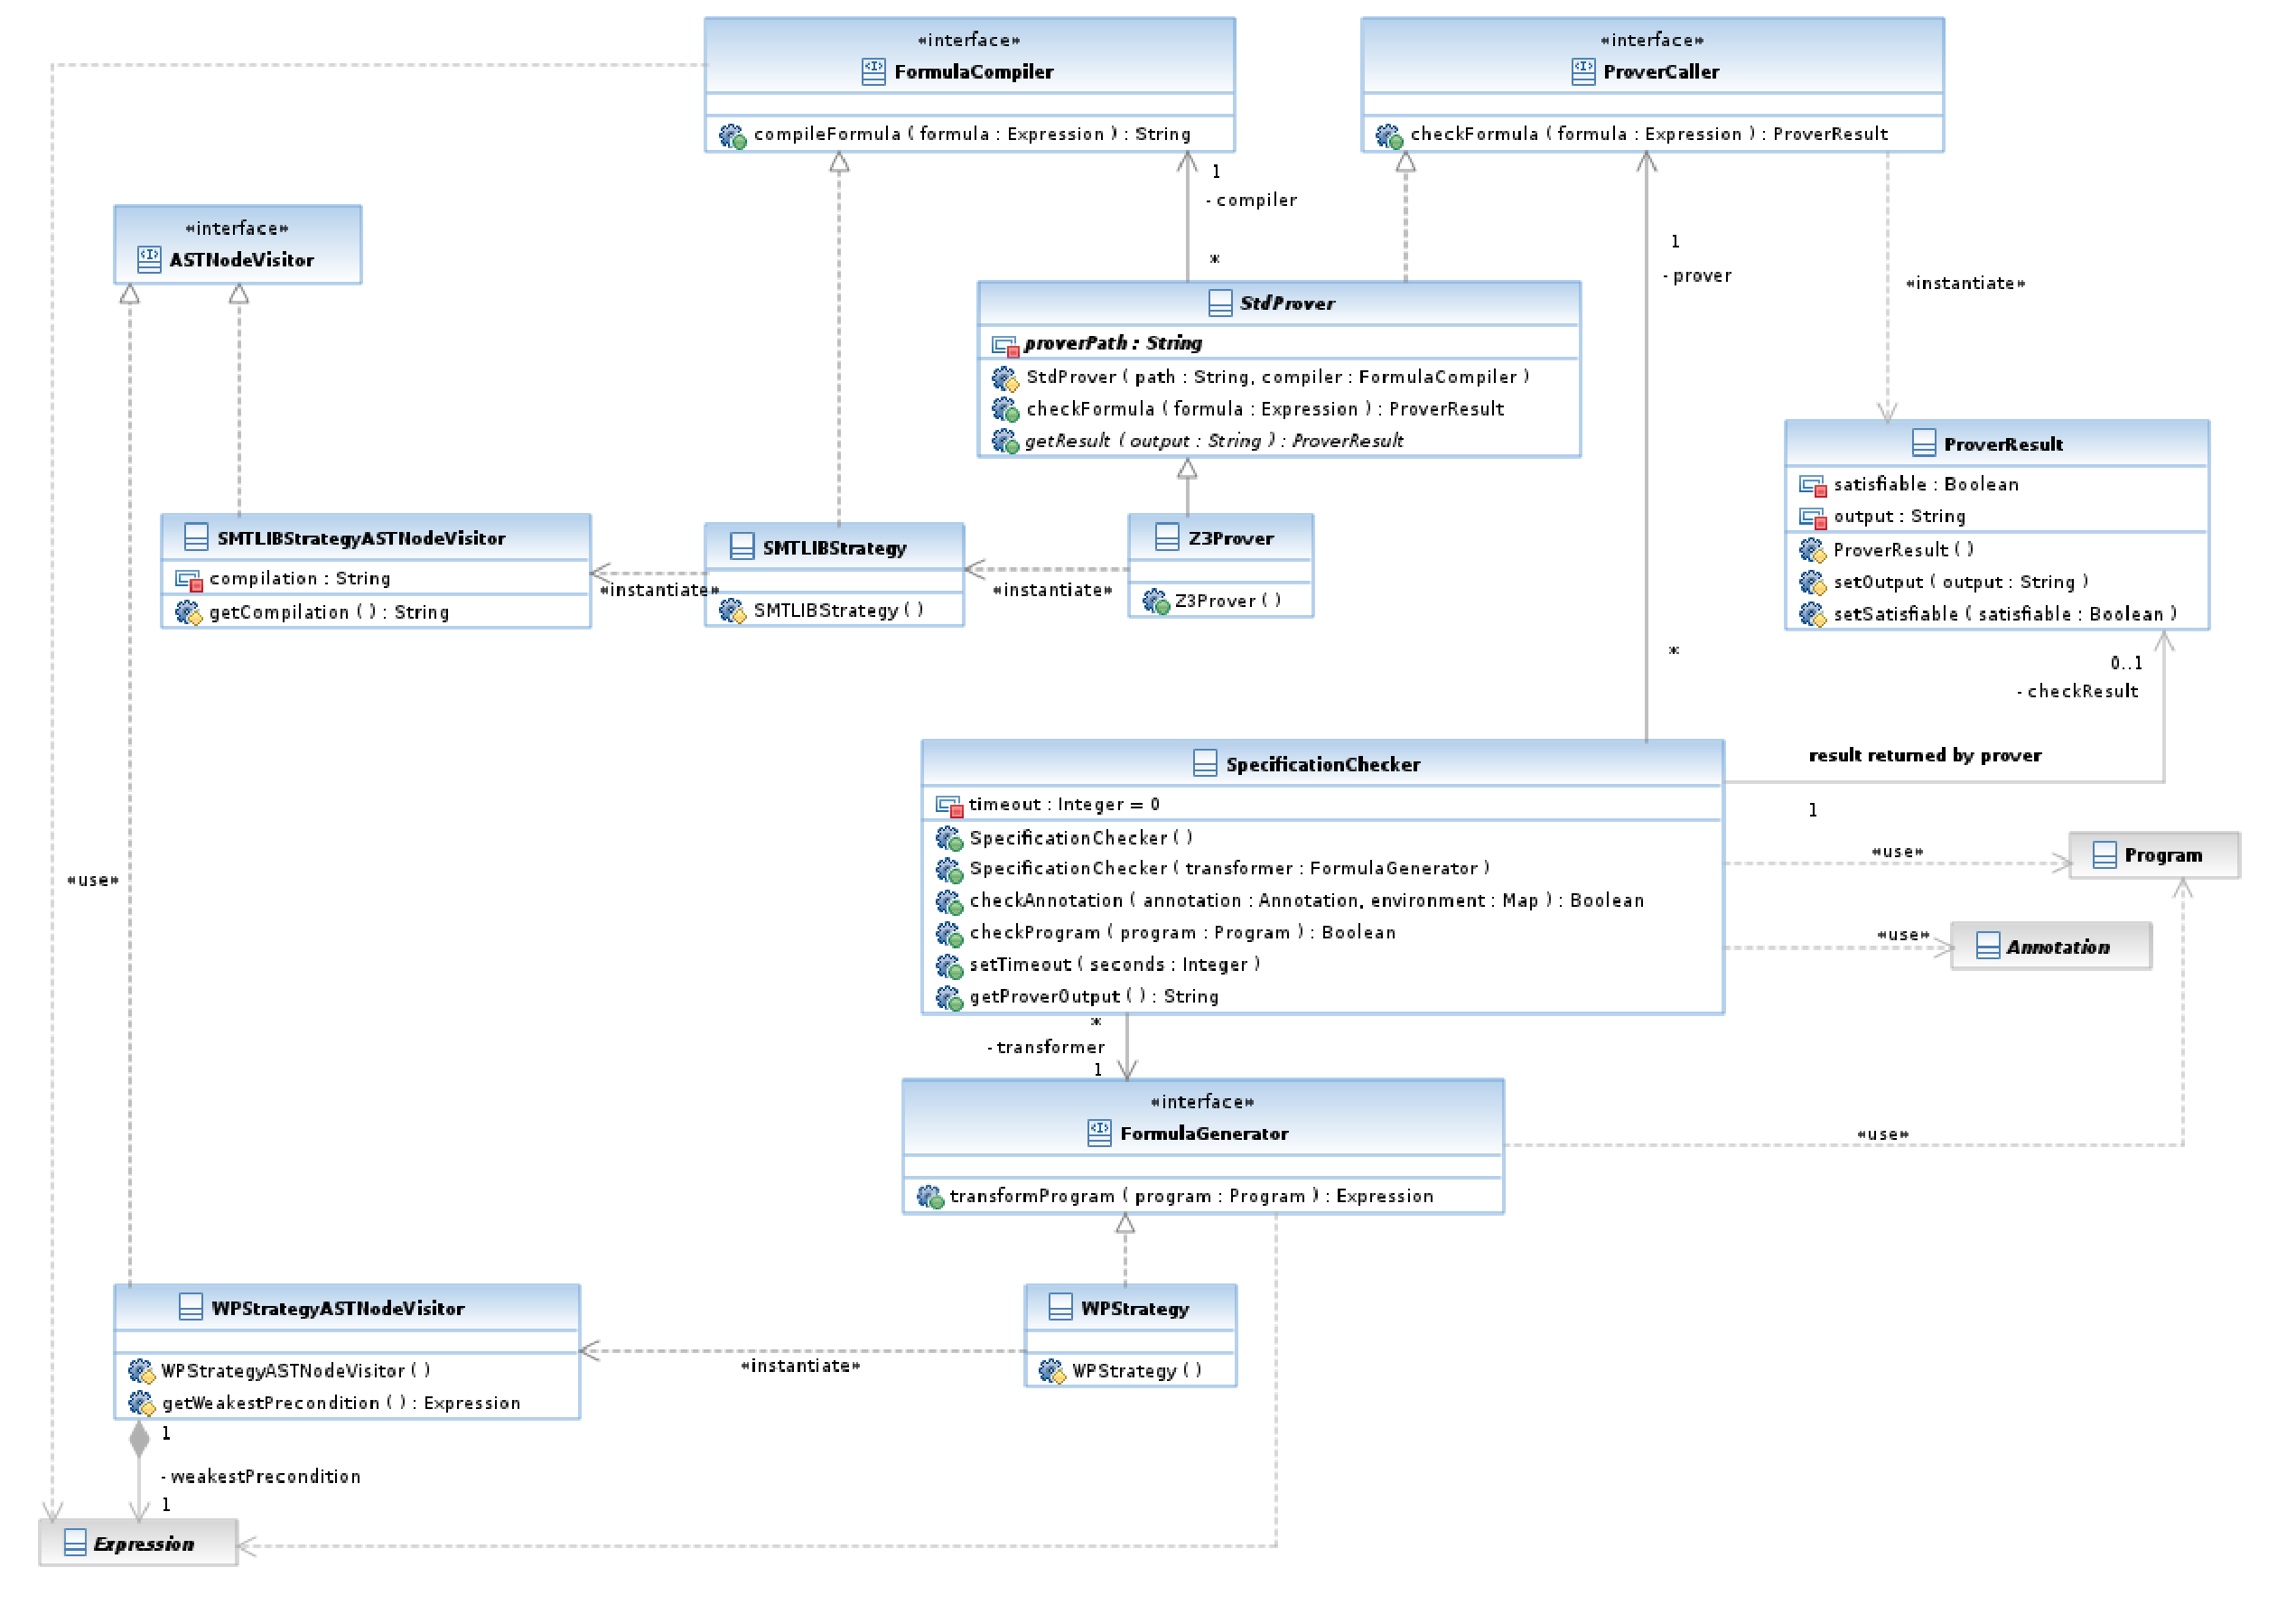
\includegraphics[width=1.5\textwidth]{diagrams/prover_component.pdf}%

    \caption{Klassendiagramm der Komponente Beweiserschnittstelle mit
    der Schnittstellenklasse \type{SpecificationChecker}}%

\end{figure}%

\subsubsection{enum Validity}%

\subsubsection{class Prover::SpecificationChecker}%

% TODO Belegung von Funktionsvariablen

Instanzen von \type{SpecificationChecker} lassen
\type{Program}-""Instanzen von einem \type{FormulaGenerator} in eine
\type{Expression} übersetzen und diese von einem \type{ProverCaller}
auf Erfülltheit für alle Belegungen der nicht initialisierten
Programmvariablen überprüfen. Das zurückgelieferte Ergebnis gibt dann
an, ob die Erfülltheit in allen diesen Fällen gegeben ist. Wenn es
Belegungen gibt, für welche die \type{Expression} nicht erfüllt ist,
wird eine zur Verifikation des Beweiserergebnisses zurückgegeben.%

% TODO nicht öffentliche Attribute

\begin{description}%
    \attr{private timeout : Integer = 0}%

    Zeit in Sekunden, nach der \texttt{check"-Program()} und
    \texttt{check"-Annotation()} zurückkehren müssen.%

    Siehe \texttt{setTimeout()}%

    \attr{private prover : ProverCaller}%

    \attr{private transformer : FormulaGenerator}%

    \attr{private checkResult : ProverResult}%

\end{description}%

% TODO öffentliche Methoden

\begin{description}%
    \method{public SpecificationChecker()}%

    \method{public SpecificationChecker(transformer : FormulaGenerator)}%

    \method{public checkProgram(program : Program) : Validity}

    Prüft mit Hilfe des Beweisers die Korrektheit des annotierten
    \type{Program}s \texttt{program}. Es wird genau dann \texttt{true}
    zurückgeliefert, wenn \texttt{program} für alle Ausführungen den
    Annotationen entspricht, und \texttt{false} sonst~(z.~B.\, wenn
    \texttt{timeout} überschritten wurde oder die Spezifikation für
    eine Ausführung nicht erfüllt wird).%

    %Siehe \texttt{getCheckResult()}%

    Siehe \texttt{FP005}%

    \method{public checkAnnotation(annotation : Annotation, environment : StringToValueMap) : Validity}

    Prüft mit Hilfe des Beweisers die Erfülltheit der Annotation
    \texttt{ann}. Es wird genau dann \texttt{true} zurückgeliefert,
    wenn \texttt{ann} im Kontext \texttt{env} erfüllt ist, und
    \texttt{false} sonst~(z.~B.\, wenn \texttt{timeout} überschritten
    wurde).%

    %Siehe \texttt{getCheckResult()}%

    Siehe \texttt{FP005}%

    %\method{public getCheckResult() : ProverResult}
    %
    %Liefert für den vorhergehenden Aufruf von %\texttt{check"-Program()}
    %oder \texttt{check"-Annotation()} das Ergebnis des Beweiseraufrufs und
    %\texttt{null}, wenn zuvor weder ein Programm noch eine Annotation
    %überprüft wurde.%

    \method{public setTimeout(seconds : Integer)}

    Setzt den Timeout für Aufrufe von \texttt{check"-Program()} und
    \texttt{check"-Annotation()} auf den Wert von \texttt{seconds}. Ist
    der angegebene Wert negativ, wird er als Null interpretiert.%

\end{description}%

\subsubsection{interface Prover::ProgramTransformer::FormulaGenerator}%

Implementierungen dieser Schnittstelle erstellen aus einem
Worthwhile-""Programmtext eine prädikatenlogische Formel. Diese Formel
soll nur dann beweisbar sein, wenn das Programm seine Spezifikation
erfüllt. Diese Korrektheit bezieht sich immer auf ein Kalkül, weshalb
Implementierungen dieser Schnittstelle meistens die Produktionsregeln
eines solchen formalen Systems kapseln.%

\begin{description}%
    \method{public transformProgram(program : Program) : Expression} %

    Liefert die aus \texttt{program} transformierte \type{Expression}
    zurück. Die Semantik der Formel ist unbestimmt, falls der
    Programmtext kein semantisch korrektes Programm beschreibt, also
    nicht ausgeführt werden kann. Ansonsten ist die zurückgelieferte
    Formel nur dann beweisbar, wenn im angewendeten Kalkül das
    WHILE-""Programm für alle Ausführungen seinen Annotationen
    entspricht.%

    Parameter \texttt{program}: Wurzelsprachelement des zu
    transformierenden Worthwhile-""Programms, d.~h.\ sowohl der
    WHILE-""Programmtext als auch dessen Annotationen sind im
    Syntaxbaum enthalten.%

\end{description}%

\subsubsection{class Prover::TheoremProver::ProverResult}%

% TODO Attribute

\begin{description}%
    \attr{private output : String}%

    \attr{private satisfiability : FormulaSatisfiability}%

\end{description}%

% TODO Methoden

\begin{description}%
    \method{protected ProverResult(satisfiability : FormulaSatisfiability, output : String)}%

\end{description}%

\subsubsection{class Prover::ProgramTransformer::WPStrategy implements ASTNodeVisitor, FormulaGenerator}%

% TODO Attribute

\begin{description}%
    \method{private weakestPrecondition : Expression}%

\end{description}%

% TODO Methoden

\begin{description}%
    \method{public transformProgram(program : Program) : Expression}%

\end{description}%

\subsubsection{interface Prover::TheoremProver::ProverCaller}%

Implementierungen dieser Schnittstelle kapseln Aufrufe eines Beweisers
für gegebene prädikatenlogische Formeln. Das Ergebnis eines Aufrufs
besteht aus der Formelerfüllbarkeit, einem Modell zur Verifikation
derselben und einer Liste semantischer Fehler.%

% TODO Methoden

\begin{description}%
    \method{public checkFormula(formula : Expression) : ProverResult}%

    Aufruf des unterstützten Beweisers für die Überprüfung der
    prädikatenlogischen Formel \texttt{formula}. Es wird nur dann
    \texttt{true} in \texttt{ProverResult\#satisfiable}
    zurückgeliefert, wenn die Formel erfüllbar ist, und \texttt{false}
    sonst. Ist \texttt{ProverResult\#satisfiable} auf \texttt{true}
    gesetzt, muss \texttt{ProverResult\#model} mit einem
    entsprechenden Modell als Zeuge und \texttt{ProverResult\#errors}
    mit einer leeren Liste initialisiert sein.%

    Parameter \texttt{formula}: Wurzelsprachelement der zu prüfenden
    prädikatenlogischen Formel.%

\end{description}%

\subsubsection{abstract class Prover::TheoremProver::StdProver extends ProverCaller}%

Instanzen von dieser Abstraktion abgeleiteter Klassen rufen Beweiser
auf, denen die zu überprüfende Formel auf der Standardeingabe
übergeben wird. Spezialisierungen dieser Klasse implementieren die
Extrahierung des Beweiserergebnisses aus der Standardausgabe.%

% TODO Attribute

\begin{description}%
    \attr{private proverPath : String}%

    \attr{private compiler : FormulaCompiler}%

\end{description}%

% TODO Methoden

\begin{description}%
    \method{protected StdProver(path : String, compiler : FormulaCompiler)}%

    Konfiguriert Instanzen so, dass der Beweiser \texttt{path} mit dem
    Formelkompilat von \texttt{compiler} für zu überprüfende
    prädikatenlogische Formeln aufgerufen wird.%

    Parameter \texttt{path}: Systempfad der ausführbaren Datei eines
    Beweisers.%

    Parameter \texttt{compiler}: Wird zur Generierung der
    Beweisereingabe aus einer angegebenen prädikatenlogischen Formel
    aufgerufen.%

    \method{public checkFormula(formula : Expression) : ProverResult}%

    Ruft den bei Objekterstellung angegebenen Beweiserpfad auf und
    füllt die Standardeingabe mit dem vom angegebenen Compiler aus
    \texttt{formula} erstellten Kompilat auf.
    \texttt{ProverResult\#satisfiable} wird auf \texttt{false}
    gesetzt, falls bei der Beweiserausführung ein Systemfehler
    aufgetreten ist, und sonst wird die Rückgabe von
    \texttt{getResult()} zurückgeliefert, welche den Inhalt der
    Standardausgabe nach Beweiseraufruf erhalten hat.%

    \method{abstract public getResult(output : String) : ProverResult}%

    Extrahiert aus \texttt{output} sowohl Ergebnis als auch Fehler
    eines Beweiseraufrufs und liefert diese Informationen in einer
    Instanz von \type{ProverResult} zurück. Kann der Inhalt von
    \texttt{output} nicht interpretiert werden, wird
    \texttt{ProverResult\#satisfiable} auf \texttt{false} gesetzt.%

    Parameter \texttt{output}: Textausgabe nach einem Beweiseraufruf.%

\end{description}%

\subsubsection{class Prover::TheoremProver::Z3Prover extends StdProver}%

% TODO Methoden

\begin{description}%
    \method{public Z3Prover()}%

    \method{public getResult(output : String) : ProverResult}%

\end{description}%

\subsubsection{interface Prover::TheoremProver::FormulaCompiler}%

Implementierungen dieser Schnittstelle übersetzen eine
\type{Expression} in die Eingabesprache eines Beweisers, sodass dieser
mit der zurückgelieferten Zeichenkette die Erfüllbarkeit der
ursprünglichen Formel prüfen und seine Ausgabe in ein verifizierendes
Modell zurückübersetzt werden kann.%

% TODO Methoden

\begin{description}%
    \method{public compileFormula(formula : Expression) : String}%

    Liefert eine Übersetzung von \texttt{formula} in eine
    Beweisersprache, sodass das erfüllende Modell eines Beweisers, der
    diese Sprache interpretiert, genau auf ein erfüllendes Modell von
    \texttt{formula} abbilden lässt~(Bedeutungserhalt).%

    %\method{protected Formula uncompileFormula(String formula)}%

\end{description}%

\subsubsection{class SMTLIBStrategy implements ASTNodeVisitor, FormulaCompiler}%

% TODO Attribute

\begin{description}%
    \attr{private compilation : String}%

\end{description}%

% TODO Methoden

%\begin{description}%
%
%\end{description}%

\subsubsection{enum FormulaSatisfiability}%

\subsection{Interaktionsentwurf}%

\begin{landscape}%
    \begin{figure}[p]%
        \vspace{-2cm}%
        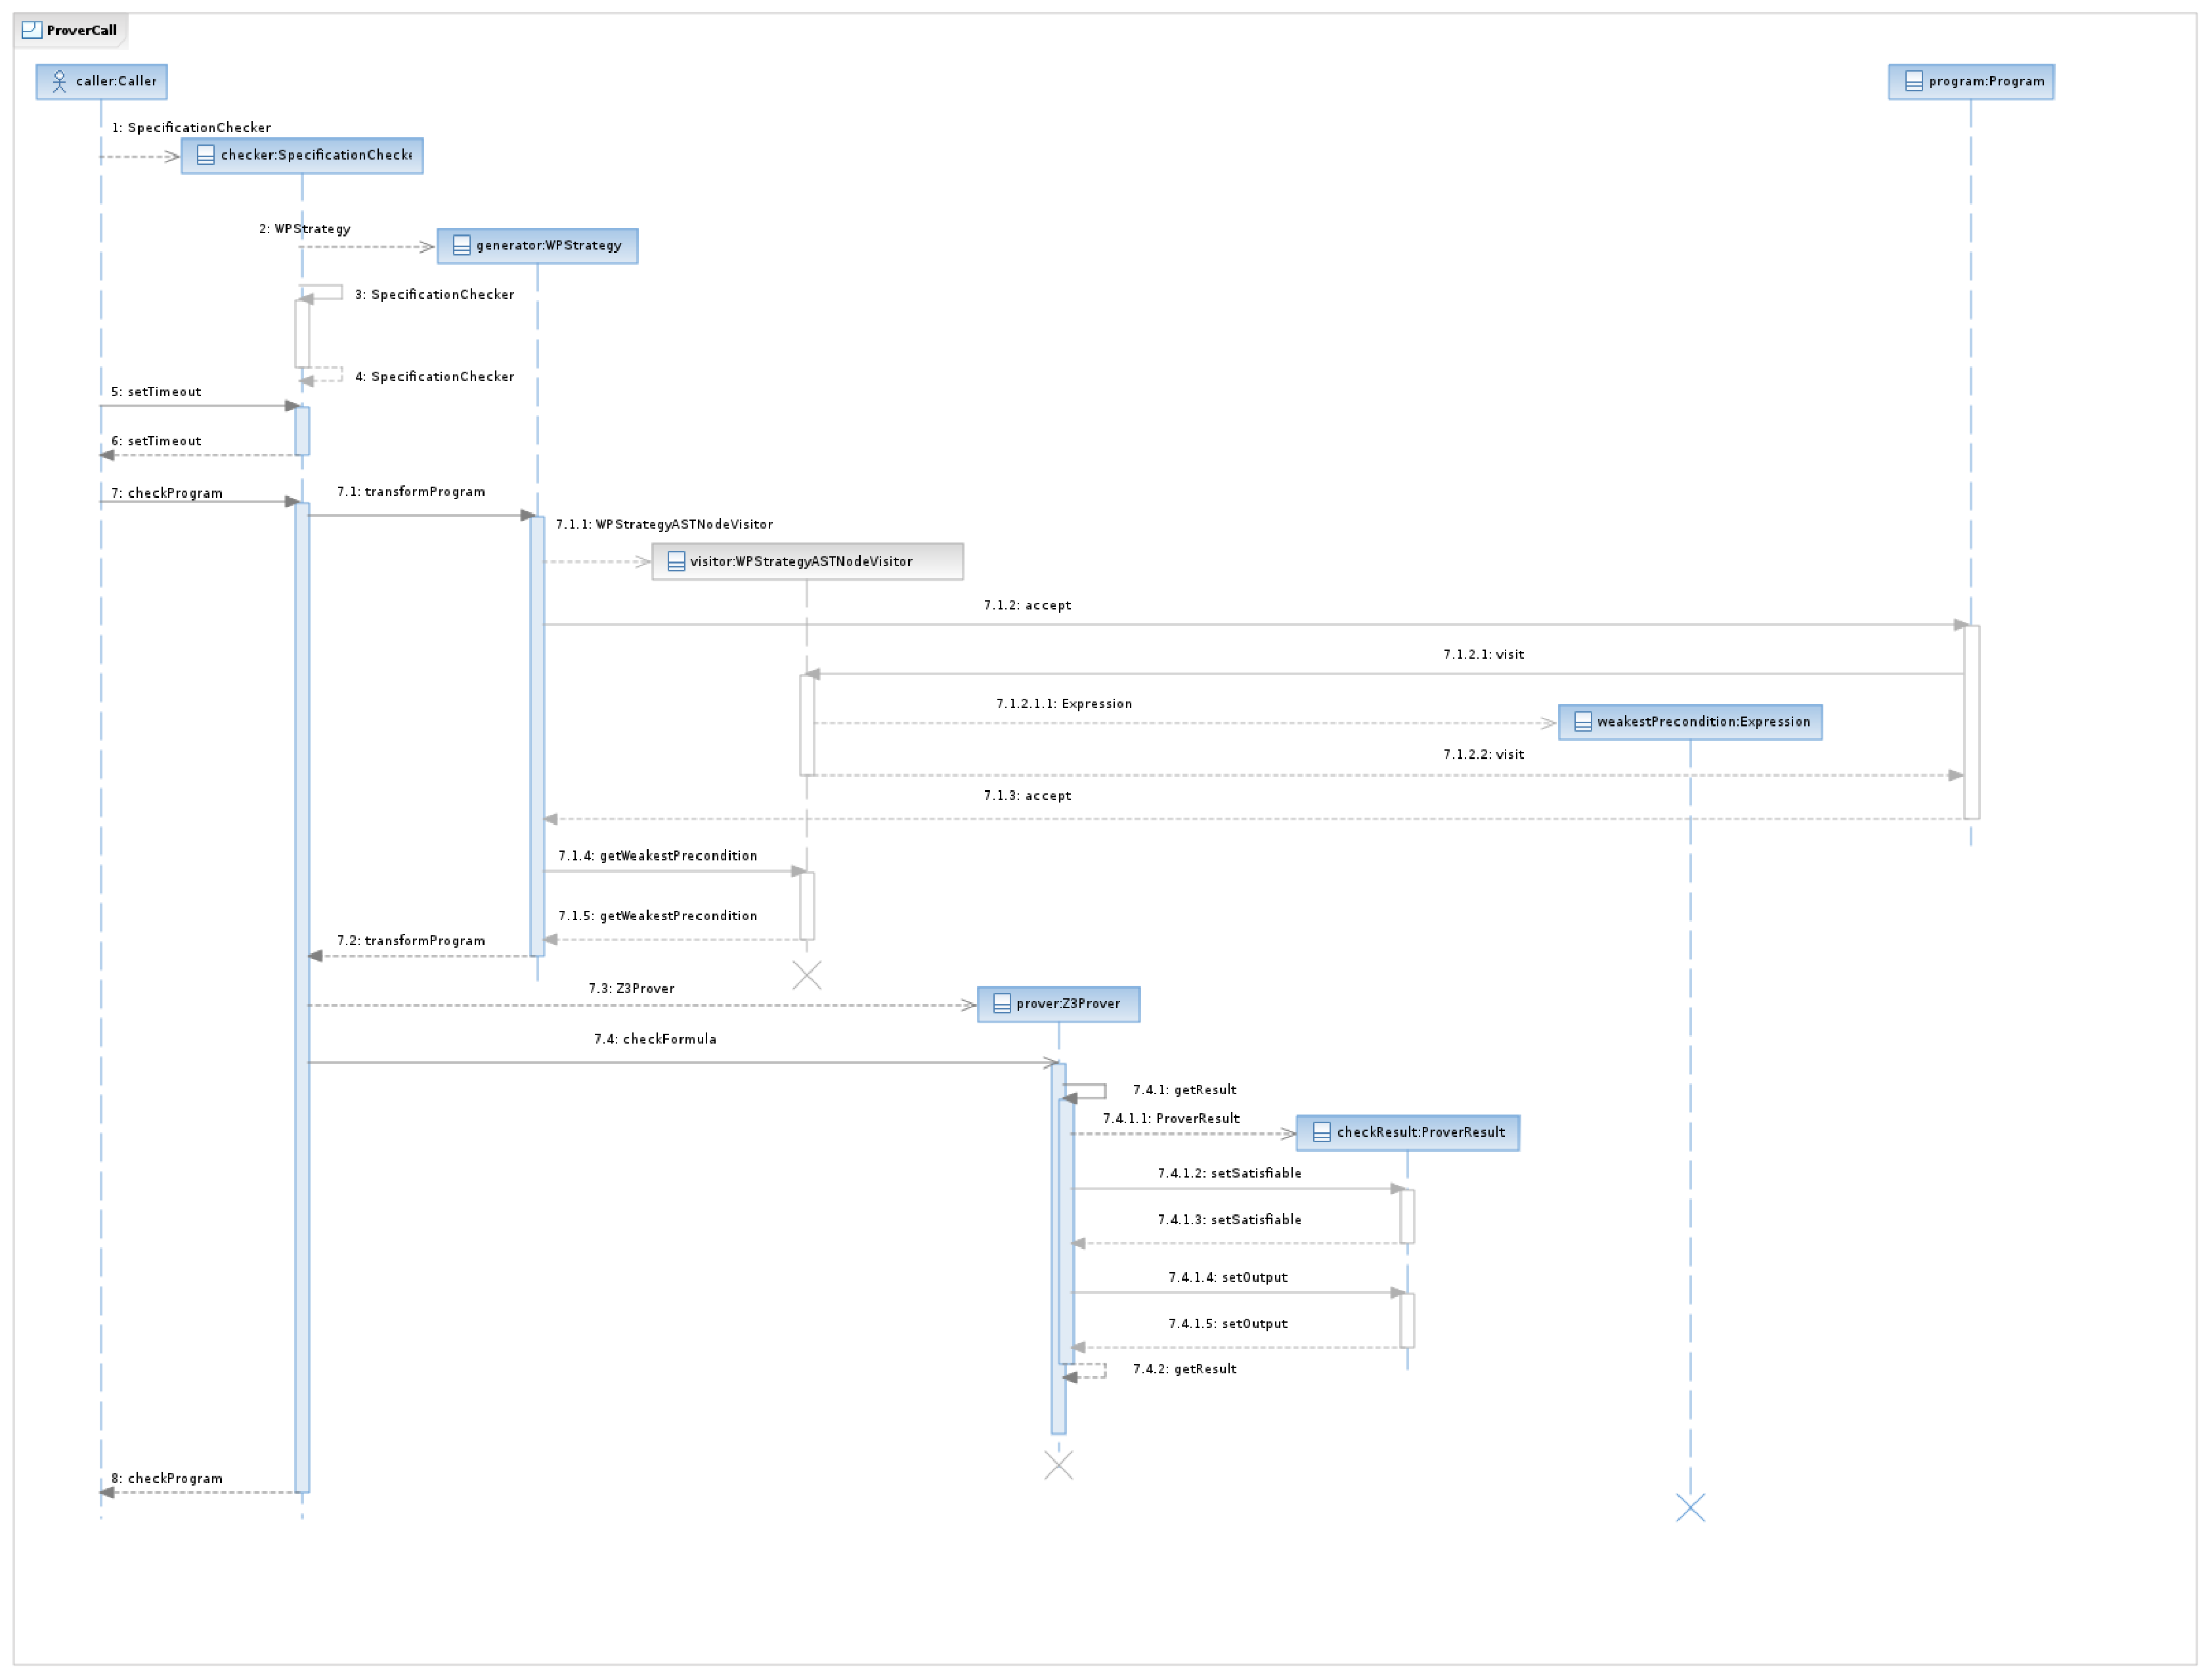
\includegraphics[height=1.2\textheight]{diagrams/programchecking_sequence.pdf}%

        \caption{Sequenzdiagramm zum Aufruf der Beweiserschnittstelle,
        um eine Programmspezifikation zu überprüfen.}%

    \end{figure}%
\end{landscape}%
